\documentclass[25pt, a0paper, portrait]{tikzposter}
\usepackage[utf8]{inputenc}
\usepackage{lmodern}
\usepackage{amsmath,amsfonts}
\usepackage{caption,subcaption,tikz}
\usepackage{lipsum} 
\usepackage{authblk}

% Define ISAE's color 
\definecolor{isaeBlue}{RGB}{37,39,117}
\definecolor{isaeCyan}{RGB}{0,173,239}

% Define ISAE color style
\definecolorstyle{isaeColorStyle} {
\definecolor{colorOne}{named}{isaeBlue}
\definecolor{colorTwo}{named}{yellow}
\definecolor{colorThree}{named}{orange}
}{
% Background Colors
\colorlet{backgroundcolor}{colorOne}
\colorlet{framecolor}{black}
% Title Colors
\colorlet{titlefgcolor}{isaeBlue}
\colorlet{titlebgcolor}{colorOne}
% Block Colors
\colorlet{blocktitlebgcolor}{isaeBlue}
\colorlet{blocktitlefgcolor}{white}
\colorlet{blockbodybgcolor}{white}
\colorlet{blockbodyfgcolor}{black}
% Innerblock Colors
\colorlet{innerblocktitlebgcolor}{isaeBlue}
\colorlet{innerblocktitlefgcolor}{black}
\colorlet{innerblockbodybgcolor}{colorThree!30!white}
\colorlet{innerblockbodyfgcolor}{black}
% Note colors
\colorlet{notefgcolor}{black}
\colorlet{notebgcolor}{colorTwo!50!white}
\colorlet{noteframecolor}{colorTwo}
}

\usetheme{Board}
\usecolorstyle{isaeColorStyle}
\useblockstyle{Default}
\usetitlestyle{Empty}
\usenotestyle{Corner}

% Write your title here
\title{
\begin{tabular}{c}
A Robust Template for ISAE \\ 
Communication and Space Exploration
\end{tabular}
}

% Fill the authors here
\author[1]{César Debeunne}
\author[2]{Justin Cano}
\author[1]{Florian Ferol}
\affil[1]{ISAE-SUPAERO}
\affil[2]{Polytechnique Montréal}

\makeatletter
\def\maketitle{\AB@maketitle}
\makeatother


\begin{document}
 
% Draw the ISAE layout
\node[above right,opacity=1,inner sep=0pt,outer sep=0pt] at (bottomleft) {\includegraphics[width=\paperwidth,height=\paperheight]{template_images/Affiche - A3.png}};
\maketitle[titletoblockverticalspace=0cm]

\begin{columns}
	
\column{0.5}
       
\block{Context}{
    \lipsum[1][]
    \begin{itemize}
        \item \lipsum[2][1]
        \item \lipsum[2][2]
        \item \lipsum[2][3]
    \end{itemize}
        
    \begin{tikzfigure}[Cute Cameras]
        %\centering
        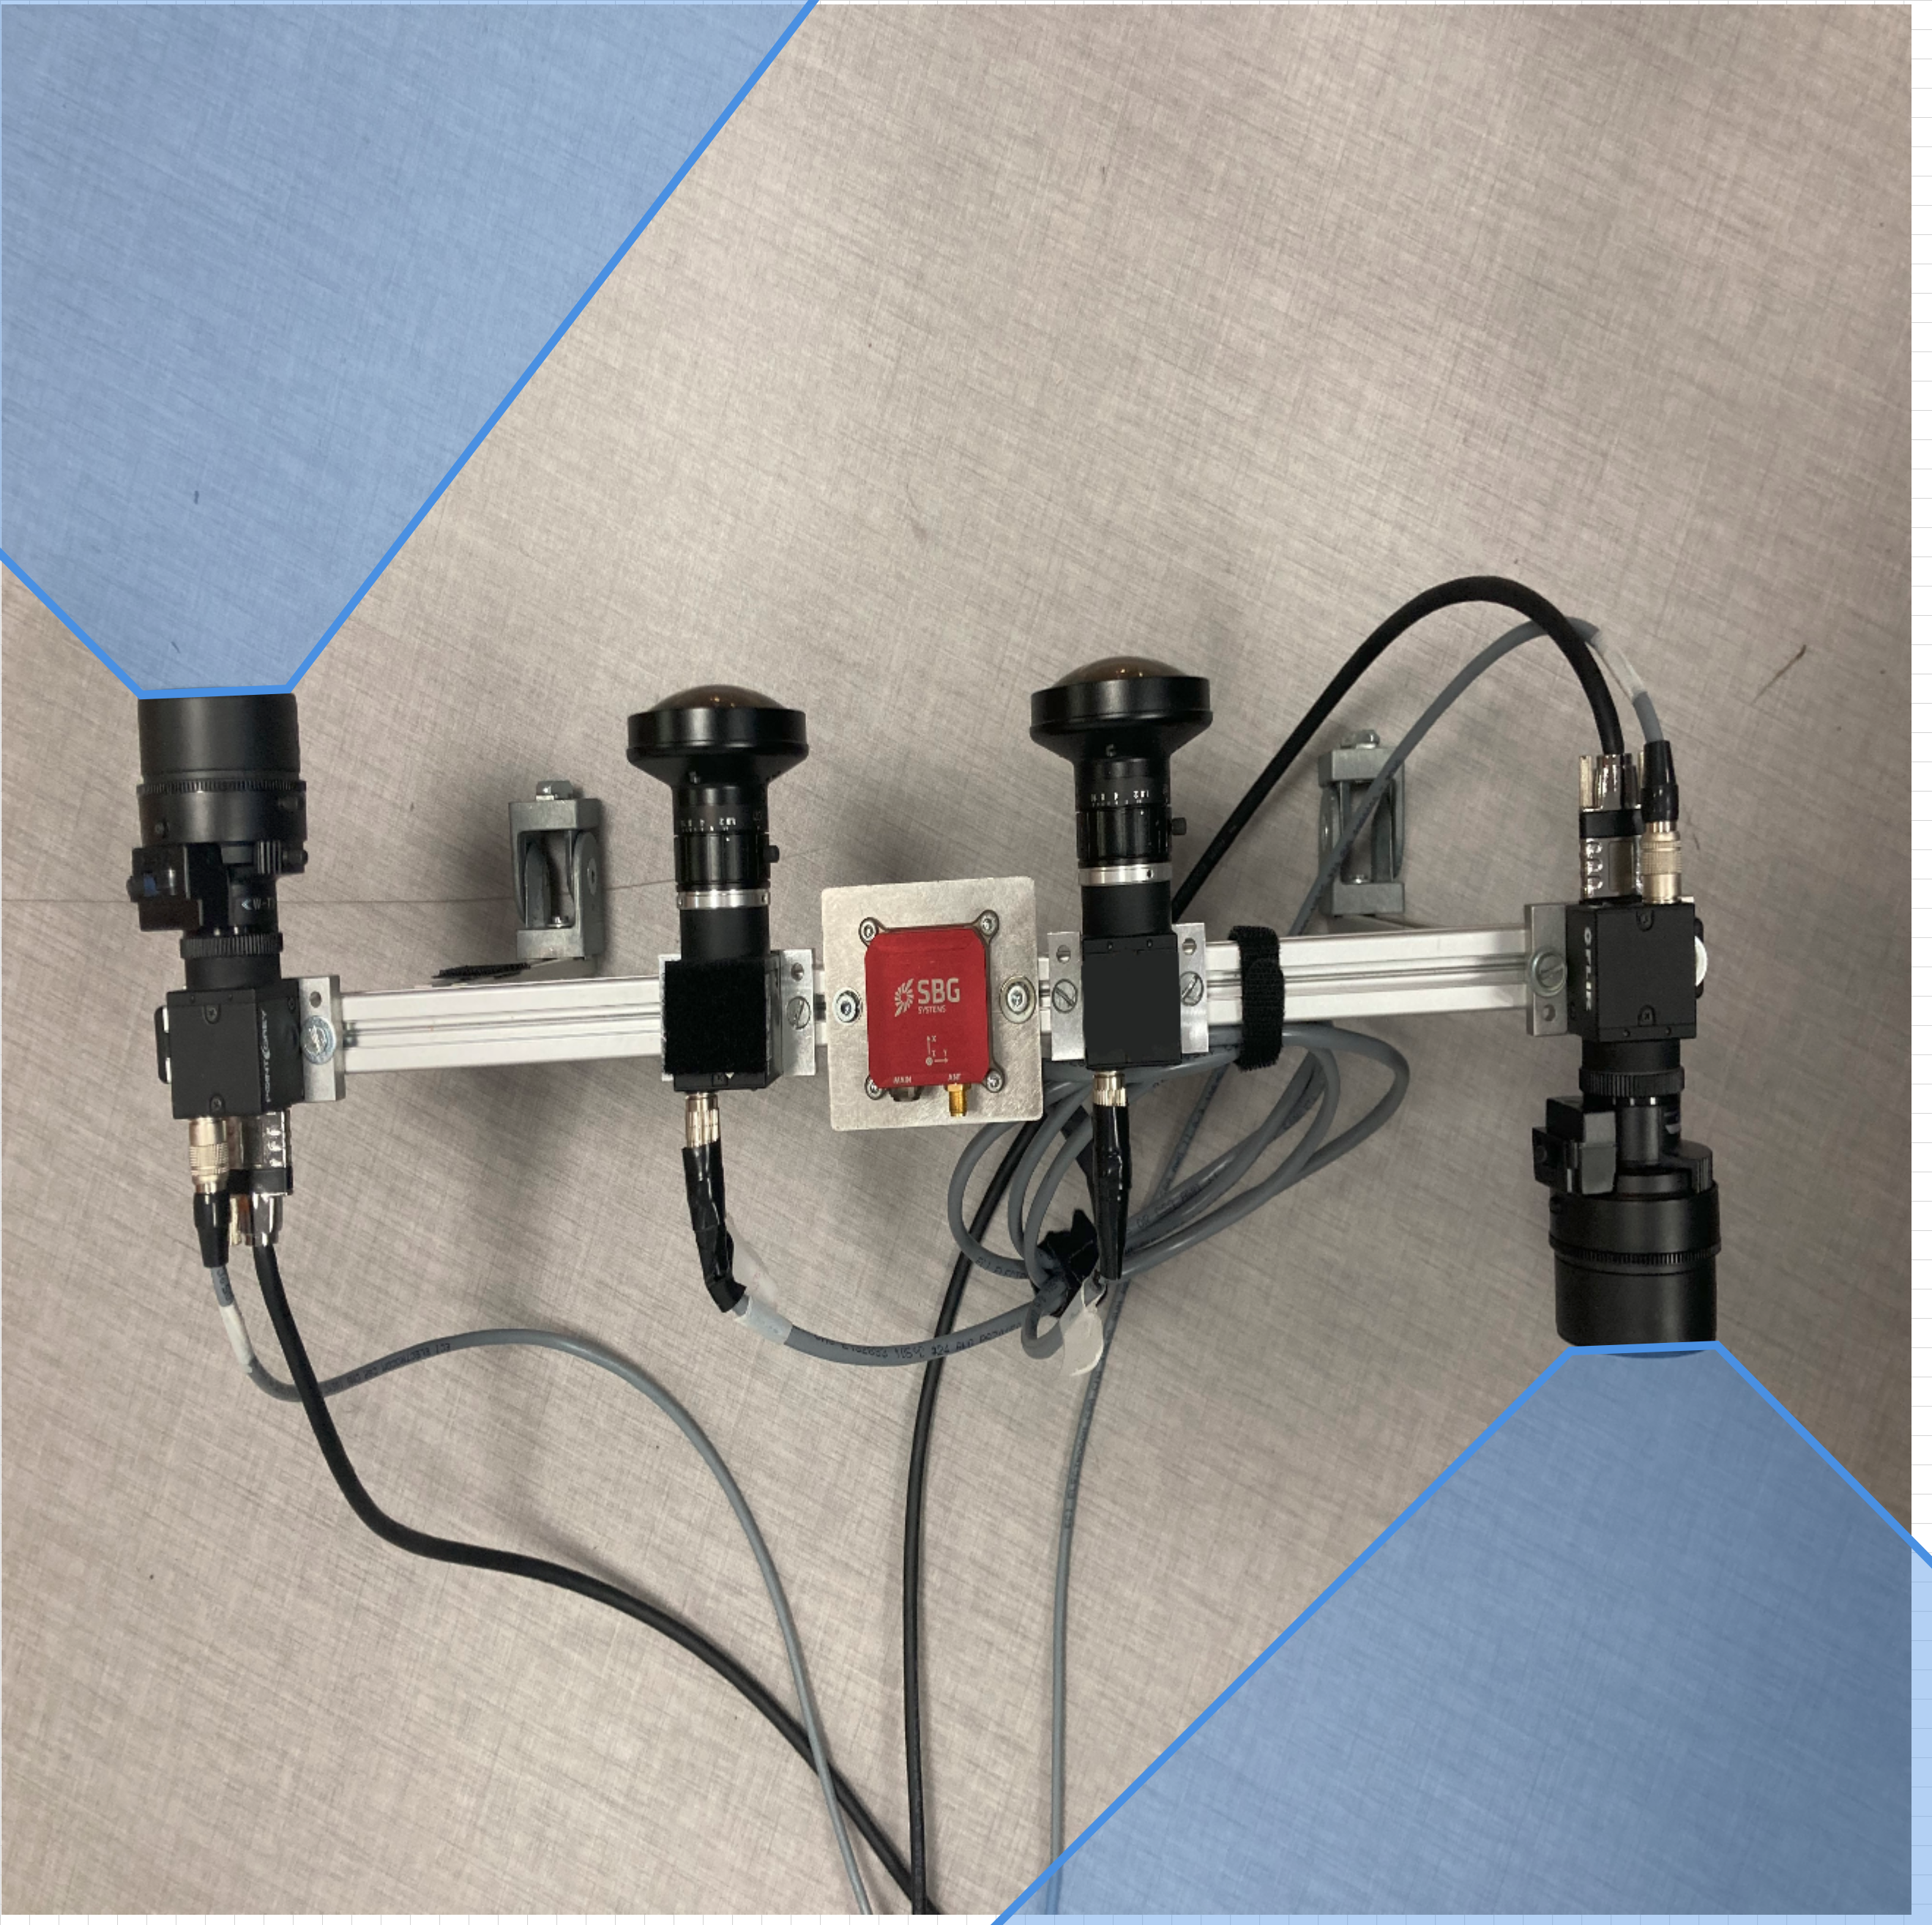
\includegraphics[width=0.7\linewidth]{images/setup.png}
        \label{fig:setup}
    \end{tikzfigure}
}


\block{Global system}{

    \lipsum[3][]
     
    \begin{tikzfigure}[Cute System.]
    	%\centering
    	\includegraphics[width=0.8\linewidth]{images/principles.pdf}
    	\label{fig:principles}
    \end{tikzfigure}
	
}

   
\column{0.5}

\block{Methodology}
{
    \lipsum[4][]

    \begin{tikzfigure}[Cute curves.]
    	%\centering
    	\includegraphics[width=0.7\linewidth]{images/scale.pdf}
    	\label{fig:scale}
    \end{tikzfigure}

    \lipsum[5][]
}


\block{Experiments}
{
    \lipsum[8][1] (\textit{cf.} figure \ref{fig:chariot}) 
    
    \begin{minipage}{0.5\linewidth}
        \vspace{1.2cm}
        \begin{tikzfigure}[Cute trajectories.]
                \centering
                \includegraphics[width=.9\linewidth]{images/trajectory_chariot1.pdf}
            \label{fig:chariot}
        \end{tikzfigure}
        
    \end{minipage}
    \begin{minipage}{0.5\linewidth}
    \vspace{2.8cm}
        \begin{tikzfigure}[Cute comparison.]
            \centering
            \includegraphics[width=\linewidth]{images/trajectory_square.pdf}
            \label{fig:square}
        \end{tikzfigure}
    \end{minipage}
    \vspace{0.5cm}
    
    \lipsum[7]
}

\block{Supervision}
{
    \lipsum[1][1] \lipsum[1][2]
}
      
\end{columns}

% Custom positionning of logos around the title
\node [opacity=1] at (0, 50)
{
\begin{minipage}[l]{0.5\linewidth}
\hspace{5cm}
\includegraphics[width=0.3\textwidth ]{template_images/isae_supaero.png}
\end{minipage}
\begin{minipage}[r]{0.5\linewidth}
\hspace{25cm}
 \includegraphics[width=0.3\textwidth ]{template_images/isae_supaero.png}
\end{minipage}            
};
   
\end{document}

